\begin{wrapfigure}{r}{0.5\textwidth}
	\begin{mdframed}
		\large{ECP ST contributes to the HPC software ecosystem through direct product development, contributions to industry and \textit{de facto} standards, and shaping the requirements, design and prototyping of products delivery by vendors and other third parties.}
	\end{mdframed}
\end{wrapfigure}
ECP ST efforts contribute to the HPC software ecosystem in a variety of ways.  Most tangible are the contributions to software products, many of which are already widely deployed and being transformed for use with Exascale systems.  However, ECP ST contributes to industry and \textit{de facto} standards efforts.  Finally, some ECP ST efforts contribute to the upstream processes of requirements, analysis, design and prototyping that informs the implementation of vendor and other third-party software products.  While they do not receive the most attention, these upstream efforts are very impactful and low cost, without a product to support.

\begin{figure}[htb]
	\begin{center}
		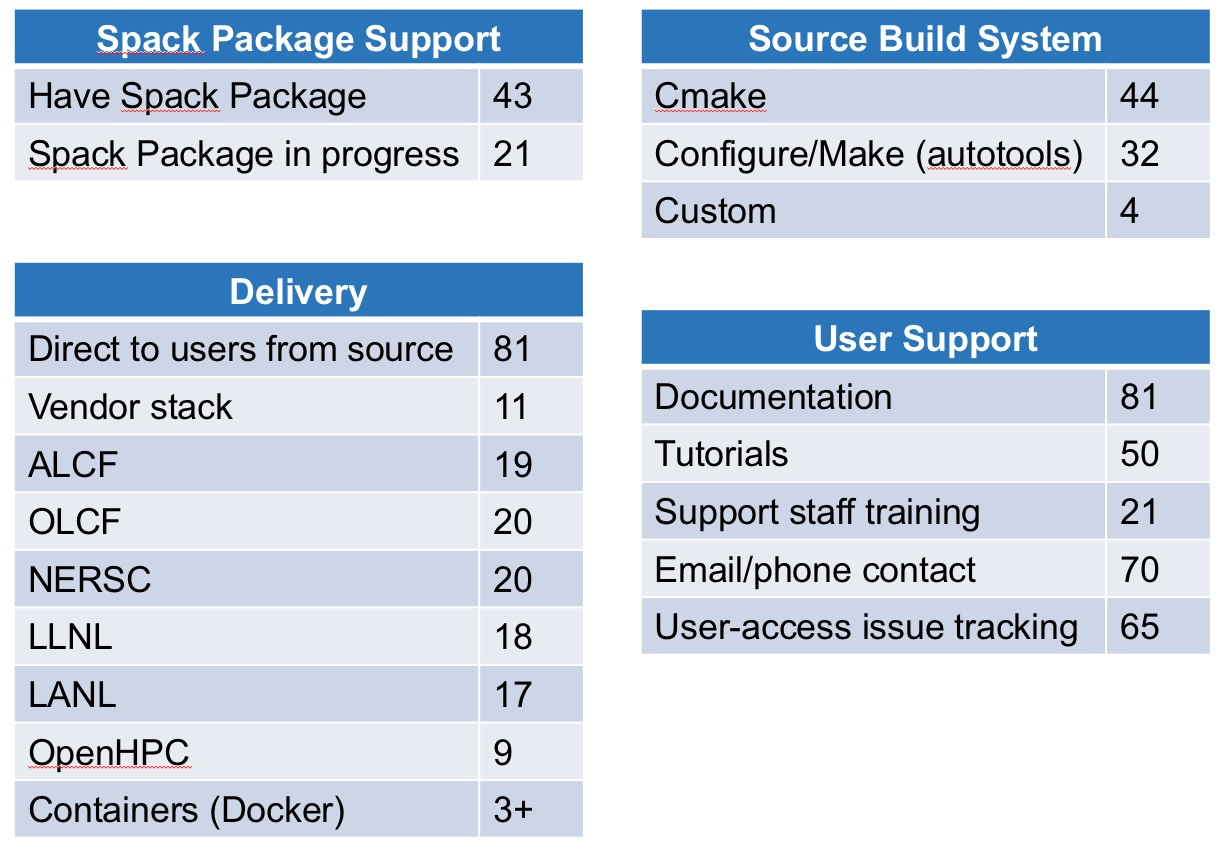
\includegraphics[width=0.7\textwidth]{ProductsOverview}

		\caption{\label{fig:productsoverview}{\small{The 54 ECP ST Projects contribute to 89 unique products.   ECP ST products are delivered to users via many mechanisms. Provides experience we can leverage across projects.  Building via Spack is required for participating in ECP ST releases: 48\% of products already support Spack.   24\% have Spack support in progress.  Use of Spack and the ECP ST SDKs will greatly improve builds from source. 81 of 89 packages support users via source builds.}}}
	\end{center}
\end{figure}
